% A two-column news report. Heading at first column. Figure at second column. Page size roughly A3.
% This code was written during 2008-2015 for Kolkata based Bengali fortnightly Khoborer Kagoj Songbadmanthan.
%============================================
\documentclass{article}
\usepackage{fontspec}
\usepackage{xunicode}
\usepackage{xltxtra}
\usepackage{multicol}
\usepackage{ragged2e}
\usepackage{wrapfig}
\usepackage{graphicx}
\usepackage[papersize={11in,18in},top=1in,bottom=1.5in,left=0.5in,right=0.5in]{geometry}
%
% These are the fonts and their variations. Baban12 and BabanBold12 fonts are custom made. Font files are provided in the directory. Ubuntu font is available in internet freely.
\newcommand\EN[1]{	
\fontsize{#1}{#1}\fontspec{Ubuntu}}
\newcommand\BN[1]{ % Normal face of the Bengali font 
\fontsize{#1}{#1}\fontspec[Script=Bengali]{Baban12}}
\newcommand\BB[1]{ % Bold face of the Bengali font 
\fontsize{#1}{#1}\fontspec[Script=Bengali]{BabanBold12}}
\newcommand\BI[1]{ % Italic face of the Bengali font 
\fontsize{#1}{#1}\fontspec[Script=Bengali, FakeSlant=0.2]{Baban12}}
\newcommand\BBI[1]{ % Bold italic face of the Bengali font 
\fontsize{#1}{#1}\fontspec[Script=Bengali, FakeSlant=0.2]{BabanBold12}}
%
%
\begin{document}
%
\begin{minipage}[t]{143mm} % A single news item should be within a minipage environment
\vspace{7mm}
\setlength{\baselineskip}{2pt}
\setlength{\parskip}{0.15ex} 
\setlength{\parindent}{10pt}
\begin{multicols}{2} % Two Column environment starts
% Heading and figure within section
[\section*{\RaggedRight
\BB{22.22}গুপ্তিপাড়ার রথযাত্রা
\\[-2mm]
\RaggedLeft
\setlength{\fboxsep}{0pt}
\setlength{\fboxrule}{0.05pt} \fbox{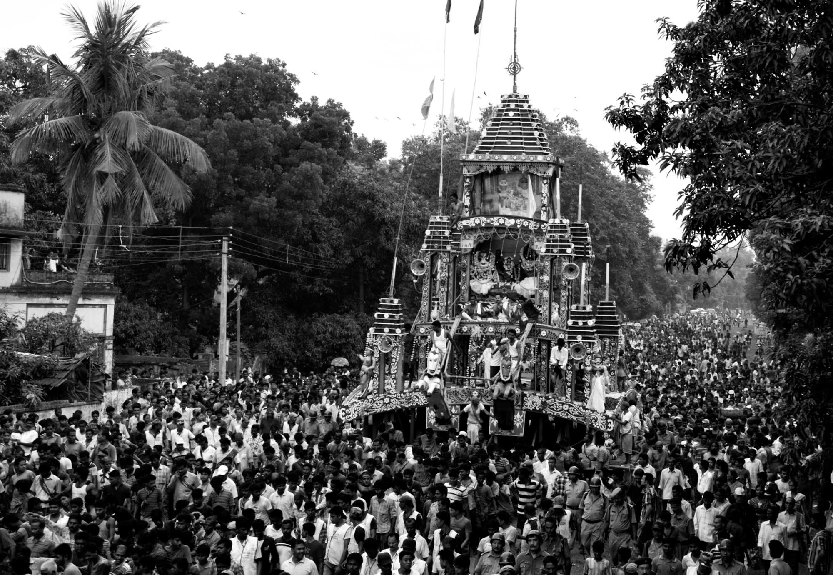
\includegraphics[width=70mm]{roth.png}}
\\[-4mm]
\parbox[t]{70mm}{\Centering\BBI{12.2545}\hspace{1mm}গুপ্তিপাড়ার এবারের রথযাত্রার ছবি বিপুল বিশ্বাসের তোলা।\hspace{1mm}} % Figure caption within parbox environment
\\[-2mm]
\rule{70mm}{0.5pt} % A horizontal line below the figure caption.
\\[0.5mm]
}]
% heading and figure insertion completed
% following three lines for adjusting multiple columns. Fourth line adjusts space between the body and the heading of the news.
\setcounter{columnbadness}{7000}
\setcounter{finalcolumnbadness}{7000}
\tolerance=2000 
.\\[-60mm]
% Reporter's name, place and date of the report.
\BBI{12.2545}বিপুল বিশ্বাস, মদনপুর, ১৭ জুলাই\EN{10}\textbullet\\[0.5mm]
% Body of the reprot
\BN{12.17}গুপ্তিপাড়া প্রধান উৎসব হল রথযাত্রা। পশ্চিমবাংলার সর্বাধিক প্রাচীন ও বৃহৎ রথগুলোর মধ্যে গুপ্তিপাড়ার রথ অন্যতম। উল্টোরথের প্রাক্কালে 'ভাণ্ডারলুঠ' উৎসব ধুমধাম করে পালিত হয় এই স্থানে। 

বাংলার মিষ্টি শিল্পের সূচনা হয়েছিল গুপ্তিপাড়াতেই। এখানেই সবার প্রথম আবিষ্কার হয়েছিল মাখা সন্দেশ। আর সেই মিশ্রণকে আকার দিয়ে নামকরণ করা হয় গুপো সন্দেশ। 

বাংলার স্থাপত্য শিল্পের অদ্ভুত নিদর্শন আজও বহন করে চলেছে এই স্থান। এখানে আছে চারটি বৈষ্ণব মন্দির। চৈতন্য, বৃন্দাবনচন্দ্র, রামচন্দ্র ও কৃষ্ণচন্দ্র -- এই চার মন্দিরের নির্মাণকাল বিভিন্ন। গুপ্তিপাড়ার মানুষ আজও একই উদ্যমে রাস, দোল ও রথযাত্রা আনন্দের সঙ্গে পালন করে চলেছে। 

রথযাত্রাকে সামনে রেখে এখানে এক গ্রাম্য মেলা অনুষ্ঠিত হয়। সমস্ত এলাকার মানুষ তাদের নিত্যপ্রয়োজনীয় সামগ্রী ধামা, কাঠা, কলসি কেনাকাটা করে। 

হাওড়া থেকে ৭৫ কিমি দূরত্বে ব্যান্ডেল কাটোয়া লাইনে অবস্থিত গুপ্তিপাড়া। হাওড়া থেকে ট্রেনে গুপ্তিপাড়া পৌঁছোতে দু-ঘন্টারও কম সময় লাগে। 
\end{multicols} 
%
\end{minipage}
%
\end{document}
